\documentclass[aspectratio=169]{beamer}
\usetheme{focus}

%\usepackage{beamerthemesplit}
%\beamertemplatenavigationsymbolsempty
\usepackage{amsmath}
\usepackage{amsthm}
\usepackage{amssymb}
\usepackage{latexsym}
\usepackage{graphicx}
\usepackage{fancybox}
\usepackage{dsfont}
\usepackage{multirow} 
\usepackage{multicol}
\usepackage{booktabs} 
\usepackage{dcolumn}
\usepackage{soul}
\usepackage[cache=false]{minted}
\usepackage{MnSymbol}
\usepackage{stmaryrd}


\DeclareMathOperator*{\argmax}{arg\,max}
\DeclareMathOperator*{\argmin}{arg\,min}

\newcommand{\X}{\mathtt{X}}
\newcommand{\Y}{\mathtt{Y}}

%\newcommand{\R}{\mathbb{R}}
%\newcommand{\E}{\mathbb{E}}
%\newcommand{\V}{\mathbb{V}}
\newcommand{\p}{\mathbb{P}}
\newcommand*\df{\mathop{}\!\mathrm{d}}
\newcommand{\del}{\partial}


% imports
\usepackage{xargs}
\usepackage{xpatch}
\usepackage{etoolbox}
\usepackage{pdflscape}
\usepackage{booktabs}
\usepackage{threeparttable}
\usepackage[skip=0.2\baselineskip]{caption}

% command for inputting raw latex
\makeatletter
\newcommand\primitiveinput[1]{\@@input #1 }
\makeatother

% common table command
\newcommandx{\tablecontent}[4]{
    \begin{threeparttable}[!ht]
        \centering
        \caption{#3}
        \vspace{-1em}
        \footnotesize
        \begin{tabular}{#1}
            \primitiveinput{../tables/#2.tex}
        \end{tabular}
        \vspace{-0.2em}
        \begin{tablenotes}[flushleft]
            #4
        \end{tablenotes}
    \end{threeparttable}
}




% \usepackage{slashbox}
\title{Lecture 3: Duration Models and Maximum Likelihood}
\author{Chris Conlon }
\institute{NYU Stern }


\newcommand{\norm}[1]{\left\lVert#1\right\rVert}
\newcommand{\R}{\mathbb{R}}
\newcommand{\E}{\mathbb{E}}
\newcommand{\V}{\mathbb{V}}
\newcommand{\ol}{\overline}
%\newcommand{\ul}{\underline}
\newcommand{\pp}{{\prime \prime}}
\newcommand{\ppp}{{\prime \prime \prime}}
\newcommand{\policy}{\gamma}


\newcommand{\fp}{\frame[plain]}

\date{\today}

\begin{document}
\maketitle

\begin{frame}{Introduction}
Consider a linear regression with $\varepsilon_i | X_i \sim N(0,\sigma^2)$
\begin{align*}
Y_{it} &= X_{i}'\beta_i + \varepsilon_{i}
\end{align*}
We've discussed the \alert{least squares estimator}:
\begin{align*}
\widehat{\beta}_{ols} &= \arg \min_{\beta} \sum_{i=1}^N (Y_i - X_i' \beta)^2\\
\widehat{\beta}_{ols} &= (\mathbf{X}'\mathbf{X})^{-1} \mathbf{X}' \mathbf{Y}
\end{align*}
\end{frame}


\begin{frame}{MLE: Example}
If we know the distribution of $\varepsilon_i$ we can construct a \alert{maximum likelihood estimator}
\begin{align*}
(\widehat{\beta}_{MLE},\widehat{\sigma}^2_{MLE} &= \arg \min_{\beta,\sigma^2} \L(\beta,\sigma^2)
\end{align*}
Where 
\begin{align*} 
L(\beta,\sigma^2) &= \prod_{i=1}^N p(y_i | x_i,\beta,\sigma^2) \\
                  &= \prod_{i=1}^N \frac{1}{\sqrt{2 \pi \sigma^2}} \exp \left[-\frac{1}{2\sigma^2}(Y_i - X_i' \beta)^2 \right]\\
l(\beta,\sigma^2) &= \sum_{i=1}^N -\frac{1}{2} \ln (2 \pi \sigma^2) - \frac{1}{2 \sigma^2}(Y_i - X_i' \beta)^2
\end{align*}
\end{frame}

\begin{frame}{MLE: FOC's}
Take the FOC's
\begin{align*}
l(\beta,\sigma^2) &= \sum_{i=1}^N -\frac{1}{2} \ln (2 \pi \sigma^2) - \frac{1}{2 \sigma^2}(Y_i - X_i' \beta)^2
\end{align*}
Where 
\begin{align*} 
\frac{ \partial l(\beta,\sigma^2) }{\partial \beta}&= \frac{1}{ \sigma^2}\sum_{i=1}^N(Y_i - X_i' \beta) = 0 \rightarrow \widehat{\beta}_{MLE}= \widehat{\beta}_{OLS}\\ 
\frac{ \partial l(\beta,\sigma^2) }{\partial \sigma^2}&= -N \frac{1}{2 \sigma^2}  -  \frac{1}{2 \sigma^4} \sum_{i=1}^N(Y_i - X_i' \beta)^2 = 0 \\
\sigma^2_{MLE} &= \frac{1}{N} \sum_{i=1}^N (Y_i - X_i' \beta)^2
\end{align*}
Note: the unbiased estimator uses $\frac{1}{N-K-1}$.
\end{frame}

\begin{frame}{MLE: General Case}
\begin{enumerate}
\item Start with the \alert{joint density of the data} $Z_1,\ldots,Z_N$ with density $f_Z(z,\theta)$
\item Construct the likelhood function of the sample $z_1,\ldots,z_n$
\begin{align*}
L(\theta) = \prod_{i=1}^N f_Z(z_i,\theta)
\end{align*}
\item Construct the \alert{log likelihood} (this has the same $\arg \max$)
\begin{align*}
l(\theta) = \sum_{i=1}^N \ln f_Z(z_i,\theta)
\end{align*}
\item Take the FOC's to find $\widehat{\theta}_{MLE}$
\begin{align*}
\theta : \frac{\partial l(\theta)}{\partial \theta} =0
\end{align*}
\end{enumerate}
\end{frame}


\begin{frame}{Example: Lancaster (1979)/ Duration Models}
Consider the following example:
\begin{itemize}
\item Unemployment durations from 479 unskilled workers
\item Characteristics: [age, local unemp rate, \alert{replacement ratio}]
% All income coming in from all sources (family support, UI benefit, supplementary benefit/ previous TH income)
\item Economic theory of job-search
\begin{itemize}
\item Receive offers arriving at some rate $\lambda(t)$ so that expected number of jobs is $\lambda(t) d\,t$.
\item Each offer is: wage $w \sim F_{W}(w)$.
\item Compare to reservation wage $w > \overline{w}(t) \rightarrow$ Accept  (otherwise reject)
\item Probability of acceptance is $1 - F_{W}(\overline{w}(t))$.
\end{itemize}
\end{itemize}
\end{frame}


\begin{frame}{Example: Constant Arrival Rate}
Now we have that $\lambda(t) d\,t= \lambda d\,t$
\begin{itemize}
\item Optimal reservation wage is constant so that $\theta = \lambda (1 - F_{W}(\overline{w}) )$
\item Implied distribution for the \alert{duration} of an unemployment \alert{spell} is \alert{exponential} 
\begin{align*}
f_Y(y) = \theta \exp(-y \theta)
\end{align*}
\item Exponential distribution is common for waiting times (\alert{memorylessness property}) $$E[Y-c | Y > c] = \frac{1}{\theta}$$
\item Distribution has mean $\frac{1}{\theta}$ and variance $\frac{1}{\theta^2}$
\end{itemize}
\end{frame}


\begin{frame}{Hazard Models}
We have defined what is known as a (constant) \alert{Hazard Model}
\begin{itemize}
\item Survivor Function: $S(y) = 1 - F_Y(y) = \exp(-y \theta)$
\item Hazard Function: $\lim_{dy \rightarrow 0^{+}} \frac{Pr(y < Y < y +dy}{Pr(y < Y)} =\frac{f_Y(y)}{S(y)} = \theta$
\item Exponential has \alert{constant hazard property}
\end{itemize}
\end{frame}

\begin{frame}{Taking the Model to Data: Perfect Data}
Suppose we have data on \alert{Exact Failure Times}
\begin{itemize}
\item This is the easy one, we see the exact unemployment duration for everyone $y_i$.
\item We can just write down the density of observing each duration for exactly $y_i$.
\begin{align*}
L(\theta) = \prod_{i=1}^N f(y_i | \theta) = \prod_{i=1}^N h(y_i| \theta) S(y_i |\theta)
\end{align*}
\end{itemize}
\end{frame}

\begin{frame}{Taking the Model to Data: Indicator}
Suppose we have data on \alert{Indicator for Survival}
\begin{itemize}
\item We see a group of people become unemployed, and we see which are still unemployed $c$ time later.
\item But we don't see anything else
\begin{align*}
L(\theta) = \prod_{i=1}^N F(c | \theta)^{d_i} (1-F(c | \theta))^{1-d_i}  = \prod_{i=1}^N (1-S(c | \theta))^{d_i} S(c | \theta)^{1-d_i}  
\end{align*}
\item This is exactly what the Survivor Function tells us about
\end{itemize}
\end{frame}



\begin{frame}{Taking the Model to Data: Censoring}
Suppose we have data on \alert{Observation over Fixed Period of Time}
\begin{itemize}
\item We see who is still unemployed after $c$ amount of time (just an indicator)
\item We see exact duration of unemployment if $y_i < c$.
\item Our data are \alert{Right Censored}
\begin{align*}
L ( \theta ) = \prod _ { i = 1 } ^ { N } f \left( y _ { i } | \theta \right) ^ { d _ { i } } \cdot S ( c | \theta ) ^ { 1 - d _ { i } } = \prod _ { i = 1 } ^ { N } h \left( y _ { i } | \theta \right) ^ { d _ { i } } \cdot S \left( y _ { i } | \theta \right) ^ { d _ { i } } \cdot S ( c | \theta ) ^ { 1 - d _ { i } }
\end{align*}
\end{itemize}
\end{frame}



\begin{frame}{Right Censoring: Continued}
\begin{itemize}
\item Helpful to define $t_i = \min(y_i,c) = d_i\cdot y_i + (1-d_i)\cdot c$ is the minimum of the actual \textit{duration} and the \alert{censoring time}
\begin{align*}
L( \theta ) = \prod _ { i = 1 } ^ { N } h \left( t _ { i } | \theta \right) ^ { d _ { i } } \cdot S \left( t _ { i } | \theta \right)
\end{align*}
\item Recall $f(y | \theta) = \theta \exp(-y \theta)$
\begin{align*}
L ( \theta ) = \theta^{\sum_{i=1}^N d_i} \exp \left(- \sum_{i=1}^N t_i \theta \right)
\end{align*}
\item the MLE is 
\begin{align*}
\hat { \theta } _ { m l e } = \sum _ { i = 1 } ^ { N } d _ { i } / \sum _ { i = 1 } ^ { N } t _ { i } = 1 / ( \overline { t } / \overline { d } ) = \overline { d } / \overline { t }\end{align*}
\end{itemize}
\end{frame}


\begin{frame}{Right Censoring: Bad Ideas}
Given the MLE $\widehat{\theta}_{MLE} = \frac{\overline{d}}{\overline{t}}$.\\

Two Bad ideas:
\begin{itemize}
\item Pretend that $y_i=c$ for people still unemployed at $c$
\begin{itemize}
    \item Pretend Censored observations $(d_i=0)$ exited $\theta = \frac{1}{\overline{t}}$. 
    \item Overestimates $\theta$ because $\overline{d} \rightarrow 1$.
\end{itemize}
\item Ignore individuals who did not exit before $c$
\begin{itemize}
    \item Ignore censored obervations and estimate $\theta = \frac{\sum d_i }{\sum d_i t_i}$. 
    \item Underestimates $\theta$ because $\sum_{i=1} t_i \rightarrow \sum_{i=1} t_i d_i$ in denominator.
\end{itemize}
\end{itemize}
\end{frame}


\begin{frame}{Taking the Model to Data: Individual Specific Censoring}
Suppose individuals differ in \alert{censoring time} $c_i$
\begin{itemize}
\item Assume $c_i \perp y_i$.
\begin{align*}
L ( \theta ) = \prod _ { i = 1 } ^ { N } f \left( y _ { i } | \theta \right) ^ { d _ { i } } \cdot S \left( c _ { i } | \theta \right) ^ { 1 - d _ { i } } = \prod _ { i = 1 } ^ { N } f \left( t _ { i } | \theta \right) ^ { d _ { i } } \cdot S \left( t _ { i } | \theta \right) ^ { 1 - d _ { i } }
= \prod _ { i = 1 } ^ { N } h \left( t _ { i } | \theta \right) ^ { d _ { i } } \cdot S \left( t _ { i } | \theta \right)
\end{align*}
\end{itemize}
\end{frame}



\begin{frame}{A Different Sampling Method}
\begin{itemize}
\item All methods assume we see individuals when they enter unemployment.
\item Suppose we just sample individuals from \alert{stock} of unemployed.
\item Imagine we draw someone who has been unmployed for $s_i=3$ weeks and finds a job after a duration of $s_i=9$ weeks
\item Let $s_i$ be duration when we first observe them, this gives:
\begin{align*}
L ( \theta ) = \prod _ { i = 1 } ^ { N } f \left( y _ { i } | \theta \right) / S \left( s _ { i } | \theta \right) = \prod _ { i = 1 } ^ { N } h \left( y _ { i } | \theta \right) \cdot \frac { S \left( y _ { i } | \theta \right) } { S \left( s _ { i } | \theta \right) }
\end{align*}
\item In general we need to know how long somone has been unemployed when we first see them. 
\item To deal with \alert{left censoring} we probably need more assumptions.
\end{itemize}
\end{frame}


\begin{frame}{Back to MLE}
Basic Setup: we know $F(z|\theta_0)$ but not $\theta_0$. We know $\theta_0 \in \Theta \subset \mathbb{R}^K$.
\begin{itemize}
\item Begin with a sample of $z_i$ from $i=1,\ldots,N$ which are I.I.D. with CDF $F(z|\theta_0)$.
\item The MLE chooses
\begin{align*}
\widehat{\theta}_{MLE} = \arg \max_{\theta} l(\theta) = \arg \max_{\theta} \sum_{i=1}^N \ln f_Z(z_i,\theta)
\end{align*}
\end{itemize}
\end{frame}


\begin{frame}{MLE: Technical Details}
\begin{enumerate}
\item Consistency. When is it true that for $\epsilon>0$?
\begin{align*}
\lim _ { N \rightarrow \infty } \operatorname { Pr } \left( \left\| \hat { \theta } _ { m l e } - \theta _ { 0 } \right\| > \varepsilon \right) = 0
\end{align*}
\item Asymptotic Normality. What else do we need to show?
\begin{align*}
\sqrt { N } \left( \hat { \theta } _ { m l e } - \theta _ { 0 } \right) \stackrel { d } { \longrightarrow } \mathcal { N } \left( 0 , - \left[ E \frac { \partial ^ { 2 } } { \partial \theta \partial \theta ^ { \prime } } \left( Z _ { i } , \theta _ { 0 } \right) \right] ^ { - 1 } \right)
\end{align*}
\item Optimization. How to we obtain $\widehat{\theta}_{MLE}$ anyway?
\end{enumerate}
\end{frame}


\begin{frame}{MLE: Example \# 1}
\begin{itemize}
\item $Z_i \sim N(\theta_0,1)$ and $\Theta = (-\infty,\infty)$. In this case:
\begin{align*}
l ( \theta ) = - N \cdot \ln ( 2 \pi ) - \sum _ { i = 1 } ^ { N } \left( z _ { i } - \theta \right) ^ { 2 } / 2
\end{align*}
\item MLE is $\widehat{\theta}_{MLE}=\overline{z}$ which is consistent for $\theta_0 = E[Z_i]$
\item Asymptotic distribution is $\sqrt{N} ( \overline{z}-\theta_0) \sim N(0,1)$.
\item Calculating mean is easy!
\end{itemize}
\end{frame}




\begin{frame}{MLE: Example \# 2}
\begin{itemize}
\item $Z_i = (Y_i, X_i)$  $X_i$ has finite mean and variance (but arbitrary distribution)
\item $(Y_i | X_i  x) \sim N(x' \beta_0, \sigma_0^2)$
\begin{align*}
\widehat{\beta}_{MLE} &= (X'X)^{-1} X'Y\\
\widehat{\sigma}^2_{MLE} &= \frac{1}{N} \sum (y_i - x_i \widehat{\beta}_{MLE})^2
\end{align*}
\item We already have shown consistency and AN for linear regression with normally distributed errors...
\end{itemize}
\end{frame}


\begin{frame}{MLE: Example \# 3}
\begin{itemize}
\item $Z_i = (Y_i, X_i)$  $X_i$ has finite mean and variance (but arbitrary distribution)
\item $Pr(Y_i=1 | X_i  x) =  \frac{e^{x' \theta_0}}{1+ e^{x'\theta_0}}$
\item Solution is the \alert{logit} model.
\item No simple MLE solution, establishing properties is not obvious...
\end{itemize}
\end{frame}

\begin{frame}{Jensen's Inequality}
Let $g(z)$ be a convex function. Then $\mathbb { E }[g(Z)] \geq g(\mathbb { E }[Z])$, with equality only in the case of a linear function.
\end{frame}

\begin{frame}{More Technical Details}
Define $Y$ as the ratio of the density at $\theta$ to the density at the true value $\theta_0$ both evaluated at $Z$
\begin{align*}
Y = \frac{f_Z(Z;\theta)}{f_Z(Z;\theta_0)}
\end{align*}
\begin{itemize}
\item Let $g(a) = -\ln(a)$ so that $g'(a) = \frac{-1}{a}$ and $g''(a) =\frac{1}{a^2}$.
\item Then by \alert{Jensen's Inequality} $\mathbb{E}[- \ln Y] \geq - \ln \mathbb{E}[Y]$.
\item This gives us
\begin{align*}
\mathbb { E }_z \left[ - \ln \left( \frac { f _ { Z } ( Z ; \theta ) } { f _ { Z } \left( Z ; \theta _ { 0 } \right) } \right) \right] \geq - \ln \left( \mathbb { E }_z \left[ \frac { f _ { Z } ( Z ; \theta ) } { f _ { Z } \left( Z ; \theta _ { 0 } \right) } \right] \right)
\end{align*}
\item The RHS is
\begin{align*}
\mathbb { E }_z \left[ \frac { f _ { Z } ( Z ; \theta ) } { f _ { Z } \left( Z ; \theta _ { 0 } \right) } \right] = \int \frac { f _ { Z } ( z ; \theta ) } { f _ { Z } \left( z ; \theta _ { 0 } \right) } \cdot f _ { Z } \left( z ; \theta _ { 0 } \right) d z = \int f _ { Z } ( z ; \theta ) d z = 1
\end{align*}
\end{itemize}
\end{frame}


\begin{frame}{More Technical Details}
Because $\log(1)=0$ this implies:
\begin{align*}
\mathbb { E }_z \left[ - \ln \left( \frac { f _ { Z } ( Z ; \theta ) } { f _ { Z } \left( Z ; \theta _ { 0 } \right) } \right) \right] \geq 0
\end{align*}
Therefore 
\begin{align*}
- \mathbb { E } \left[ \ln f _ { Z } ( Z ; \theta ) \right] &+ \mathbb { E } \left[ \ln f _ { Z } \left( Z ; \theta _ { 0 } \right) \right] \geq 0\\
\mathbb { E } \left[ \ln f _ { Z } \left( Z ; \theta _ { 0 } \right) \right] &\geq \mathbb { E } \left[ \ln f _ { Z } ( Z ; \theta ) \right]
\end{align*}
\begin{itemize}
\item We maximize the expected value of the log likelihood at the true value of $\theta$!
\item Helpful to work with $E[\log f(z; \theta)]$ sometimes.
\end{itemize}
\end{frame}


\begin{frame}{Information Matrix Equality}
We can relate the \alert{Fisher Information} to the Hessian of the log-likelihood
\begin{align*}
\mathcal { I } \left( \theta _ { 0 } \right) = - \mathbb { E } \left[ \frac { \partial ^ { 2 } \ln f } { \partial \theta \partial \theta } \left( z ; \theta _ { 0 } \right) \right] = \mathbb { E } \left[ \frac { \partial \ln f } { \partial \theta } \left( z ; \theta _ { 0 } \right) \cdot \frac { \partial \ln f } { \partial \theta ^ { \prime } } \left( z ; \theta _ { 0 } \right) \right]
\end{align*}
\begin{itemize}
    \item This is sometimes known as the \alert{outer product of scores}.
    \item This matrix is \alert{negative definite}
\end{itemize}
\end{frame}


\begin{frame}{Proof}
\begin{align*}
1 = \int _ { z } f _ { Z } ( z ; \theta ) d z \Rightarrow 0 = \frac { \partial } { \partial \theta } \int _ { z } f _ { Z } ( z ; \theta ) d z
\end{align*}
With some regularity conditions
\begin{align*}
0 = \int _ { z } \frac { \partial f _ { Z } } { \partial \theta } ( z ; \theta ) d z = \underbrace{\int _ { z } \frac { \partial \ln f _ { Z } } { \partial \theta } ( z ; \theta ) \cdot f _ { Z } ( z ; \theta ) d z}_{\mathbb { E } \left[ \frac { \partial \ln f _ { Z } } { \partial \theta } \left( z ; \theta _ { 0 } \right) \right]}
\end{align*}

\begin{itemize}
    \item This gives us the FOC we needed.
    \item Can get information identity with another set of derivatives.
    \end{itemize}
\end{frame}


\begin{frame}{The Cramer-Rao Bound}
We can relate the \alert{Fisher Information} to the Hessian of the log-likelihood
\begin{align*}
\mathcal { I } ( \theta ) = - \mathbb { E } \left[ \frac { \partial ^ { 2 } \ln f } { \partial \theta \partial \theta ^ { \prime } } ( Z | \theta ) \right]
\end{align*}
It turns out this provides a bound on the variance
\begin{align*}
\operatorname { Var } ( \hat { \theta } ( Z ) ) \geq \mathcal { I } \left( \theta _ { 0 } \right) ^ { - 1 }
\end{align*}
Because we can't do better than Fisher Information we know that MLE is most efficient estimator!
\end{frame}

\begin{frame}{MLE: Discussion}
Tradeoffs
\begin{itemize}
\item How does this compare to GM Theorem?
\item If MLE is most efficient estimate, why ever use something else?
\end{itemize}
\end{frame}

\begin{frame}{Exponential Example}
\begin{align*}
f _ { Y | X } ( y | x , \beta _ { 0 } ) =  { e } ^ { x ^ { \prime } \beta _ { 0 } } \exp \left( - y  { e } ^ { x ^ { \prime } \beta _ { 0 } } \right)
\end{align*}
With log likelihood
\begin{align*}
l( \beta ) = \sum _ { i = 1 } ^ { N } \ln f _ { Y | X } \left( y _ { i } | x _ { i } , \beta \right) = \sum _ { i = 1 } ^ { N } X _ { i } ^ { \prime } \beta - y _ { i } \cdot \exp \left( x _ { i } ^ { \prime } \beta \right)
\end{align*}
And Score, Hessian, and Information Matrix:
\begin{align*}
\mathcal { S } ( y , x , \beta ) &= x ^ { \prime } \left( 1 - y \exp \left( x ^ { \prime } \beta \right) \right)\\
\mathcal { H } ( y , x , \beta ) &= - y x x ^ { \prime } \exp \left( x ^ { \prime } \beta \right)\\
\mathcal { I } \left( \beta _ { 0 } \right) &= \mathbb { E } \left[ Y X X ^ { \prime } \exp \left( X ^ { \prime } \beta _ { 0 } \right) \right] = \mathbb { E } \left[ X X ^ { \prime } \right]
\end{align*}
\end{frame}


\section*{Computing Maximum Likelihood Estimators}

\begin{frame}{Newton's Method}
Start with the objective $Q(\theta) = - l(\theta)$:
\begin{itemize}
\item Approximate $Q(\theta)$ around some initial guess $\theta_0$ with a quadratic function
\item Minimize the quadratic function (because that is easy) call that $\theta_1$
\item Update the approximation and repeat.
\begin{align*}
\theta_{k+1} = \theta_k - \left[ \frac{\partial^2 Q}{\partial \theta \partial \theta'} \right]^{-1}\frac{\partial Q}{\partial \theta}(\theta_k)
\end{align*}
\item An important property is whether the \alert{Hessian Matrix} is positive semi-definite at all $\theta$.
\item In that case the problem is \alert{globally convex} and has a \alert{unique maximum} that is easy to find.
\end{itemize}
\end{frame}

\begin{frame}{Back to Duration Example}
Let $Z_i = (Y_i,X_i)$ and assume that $(Y_i | X_i = X) ~ Exp(\lambda)$ so that hazard rate is $exp[x'\beta_0]$ and $E[Y_i | X_i=x] = \exp(-x_i'\beta_0)$. This extends the exponential duration model to include covariates $x_i'\beta$
\begin{align*}
f ( y | x , \beta _ { 0 } ) = { e } ^ { x ^ { \prime } \beta _ { 0 } } \exp \left( - y  { e } ^ { x ^ { \prime } \beta _ { 0 } } \right)
\end{align*}
This gives the log-likelihood
\begin{align*}
l ( \beta ) = \sum _ { i = 1 } ^ { N } \ln f \left( y _ { i } | x _ { i } , \beta \right) = \sum _ { i = 1 } ^ { N } x _ { i } ^ { \prime } \beta - y _ { i } \cdot \exp \left( x _ { i } ^ { \prime } \beta \right)
\end{align*}
With derivatives (No analytic solution!)
\begin{align*}
\frac { \partial L } { \partial \beta } ( \beta ) &= \sum _ { i = 1 } ^ { N } x _ { i } \cdot \left( 1 - y _ { i } \cdot \exp \left( x _ { i } ^ { \prime } \beta \right) \right)\\
\frac { \partial ^ { 2 } L } { \partial \beta \partial \beta ^ { \prime } } ( \beta ) &= - \sum _ { i = 1 } ^ { N } x _ { i } x _ { i } ^ { \prime } \cdot y _ { i } \cdot \exp \left( x _ { i } ^ { \prime } \beta \right)
\end{align*}
This is PD if $\sum x_i x_i'$
\end{frame}

\begin{frame}{Newton's Method}
We can generalize to Quasi-Newton methods:
\begin{align*}
\theta_{k+1} = \theta_k -  \lambda_k \underbrace{\left[ \frac{\partial^2 Q}{\partial \theta \partial \theta'} \right]^{-1}}_{A_k} \frac{\partial Q}{\partial \theta}(\theta_k)
\end{align*}
Two Choices:
\begin{itemize}
\item Step length $\lambda_k$
\item Step direction $d_k=A_k \frac{\partial Q}{\partial \theta}(\theta_k)$
\item Often rescale the direction to be unit length $\frac{d_k}{\norm{d_k}}$.
\item If we use $A_k$ as the true Hessian and $\lambda_k=1$ this is a \alert{full Newton step}.
\end{itemize}
\end{frame}

\begin{frame}{Newton's Method: Alternatives}
Choices for $A_k$
\begin{itemize}
\item $A_k= I_{k}$ (Identity) is known as \alert{gradient descent} or \alert{steepest descent}
\item BHHH. Specific to MLE. Exploits the \alert{Fisher Information}.
\begin{align*}
A _ { k } 
&= \left[ \frac { 1 } { N } \sum _ { i = 1 } ^ { N } \frac { \partial \ln f } { \partial \theta } \left( \theta _ { k } \right) \frac { \partial \ln f } { \partial \theta ^ { \prime } } \left( \theta _ { k } \right) \right] ^ { - 1 }\\
&=- \mathbb { E } \left[ \frac { \partial ^ { 2 } \ln f } { \partial \theta \partial \theta ^ { \prime } } \left( Z , \theta ^ { * } \right) \right] 
= \mathbb { E } \left[ \frac { \partial \ln f } { \partial \theta } \left( Z , \theta ^ { * } \right) \frac { \partial \ln f } { \partial \theta ^ { \prime } } \left( Z , \theta ^ { * } \right) \right]
\end{align*}
\item Alternatives \alert{SR1} and \alert{DFP} rely on an initial estimate of the Hessian matrix and then approximate an update to $A_k$.
\item Usually updating the Hessian is the costly step.
\item Non invertible Hessians are bad news.
\end{itemize}
\end{frame}

\section{Back to Duration Models}

\begin{frame}
\frametitle{Overview}
Simple cases:
\begin{itemize}
\item The simplest cases are single irreversible transitions
\begin{itemize}
\item Alive $\rightarrow$ Dead
\item Working $\rightarrow$ Failure
\end{itemize}
\item Other easy cases are ``resetting'' processes:
\begin{itemize}
\item Employed $\rightarrow$ unemployed for zero weeks, one week, etc.
\item Healthy $\rightarrow$ Sick Day 1, Sick Day 2, etc.
\item Not on strike $\rightarrow$ Strike Day 1, Strike Day 2, etc.
\end{itemize}
\item Let's start with these before we worry about multivariate outcomes or more complicated cases.
\end{itemize}
\end{frame}


\begin{frame}
\frametitle{Decisions}
Have to make some decisions first
\begin{enumerate}
\item Do we model \alert{spell length} directly or \alert{probability of transition}?
\begin{itemize}
\item Most of the time we want to work with probability of transition.
\item If we work with probability of transition, we have to pay attention to \alert{frequency}
\end{itemize}
\item What outcomes do we measure: \alert{stocks}? or \alert{flows}?
\begin{itemize}
\item Do we measure the number of people who lose/find jobs?
\item Do we measure the number of unemployed people each month?
\end{itemize}
\item Is the data \alert{truncated} or \alert{censored}?
\begin{itemize}
\item People who are still alive are not in the dataset!
\end{itemize}
\end{enumerate}
For now we will think about \alert{single-spells}, and measure them using \alert{flow data}.
\end{frame}

\begin{frame}
\frametitle{Examples}
There are lots of different names (depending on your discipline):
\begin{itemize}
\item Life table analysis
\item Hazard Analysis
\item transition analysis
\item survival analysis
\item failure time analysis
\end{itemize}
Examples:
\begin{itemize}
\item How long does a government last?
\item How long does a part last?
\item How long before a firm adopts a new technology?
\item How long do marriages last?
\item How long before criminals re-offend?
\end{itemize}
\end{frame}

\begin{frame}
\frametitle{Start with a Graph!}
\begin{center}
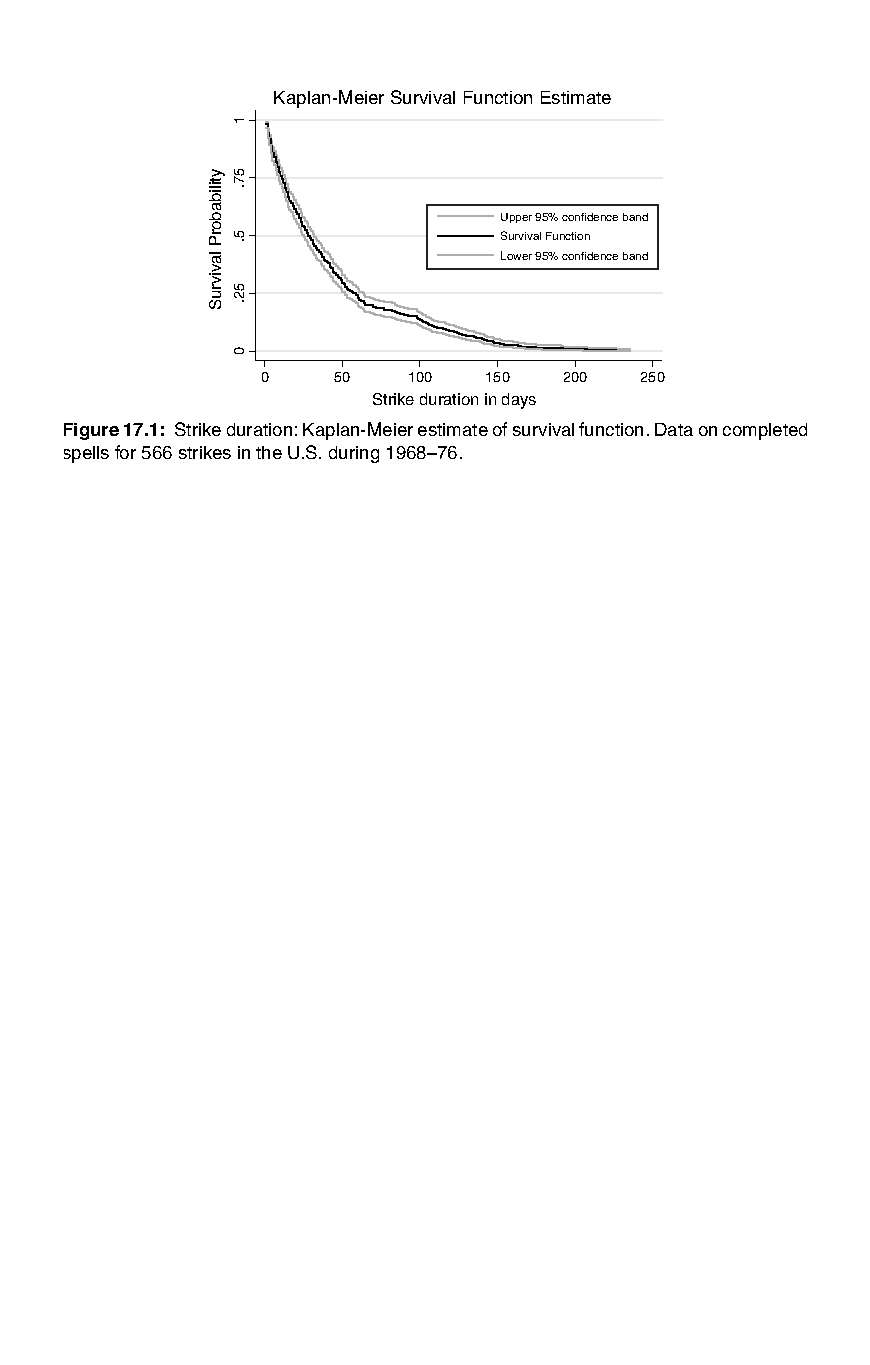
\includegraphics[width=4.5in]{./resources/figure17-1.pdf}
\end{center}
\end{frame}

\begin{frame}
\frametitle{What did we just plot?}
The \alert{empirical survival function}
\begin{itemize}
\item We ignored any covariates, including calendar time.
\item The x-axis was the duration
\item The y-axis was the fraction of observations still alive ``alive'' after $x$ periods.
\item If nothing is infinitely lived then the graph always starts at $1$ and always ends at zero.
\item If things are infinitely lived we call the duration distribution \alert{defective}.
\end{itemize}
\end{frame}

\begin{frame}
\frametitle{Parametric}
Let's start with some deeply parametric stuff
\begin{itemize}
\item density function: $f(t) = d F(t) / dt$: unconditional probability of instantaneous failure
\item CDF: $F(t) = Pr(T \leq t) = \int_0^{\infty} f(s) d s$. (Probability that spell is less than length $t$).
\item Survival Function: $S(t) = 1- F(t) = Pr( T > t)$. This has the nice property that it integrates to expected duration $\int_0^{\infty} S(t) d t = E[T]$.
\item Hazard Function: $\lambda(t)  = \lim_{\Delta t \rightarrow 0} \frac{Pr[t \leq T < t+ \Delta t | T \geq t]}{\Delta t} = \frac{f(t)}{S(t)}$.
\item \alert{All of these functions represent the same information!}
\end{itemize}
\end{frame}

\begin{frame}
\frametitle{More about hazard functions}
\small
\begin{itemize}
\item Hazard is conditional probability of leaving unemployment after being unemployed for $t$.
\item Hazard is percentage change in survivor function $S(t)$
\item Hazard also gives us the distribution of duration $T$:
\begin{eqnarray*}
\lambda(t) = - \frac{\partial \log S(t)}{\partial t}, \quad
S(t) = \exp \left[ - \int_0^{\infty} \lambda(u) d u \right]
\end{eqnarray*}
\item Often we'd like to estimate $\lambda(t | x)$ instead of $E[T | x]$ especially since we often have \alert{censored} data so that  $\lambda(t | x)$ is still well defined but $E[T | x]$ is not.
\item In practice  $\lambda(t | x)$ can be tricky to estimate (especially since it may contain zeros at some $t$ in finite sample. Solution: \alert{Cumulative Hazard Function}.
\begin{eqnarray*}
\Lambda(t) = \int_0^{\infty} \lambda(s) d s = - \log S(t)
\end{eqnarray*}
\item Just like we preferred to estimate CDF instead of PDF!
\end{itemize}
\end{frame}

\begin{frame}
\frametitle{Summary Table}
\begin{center}
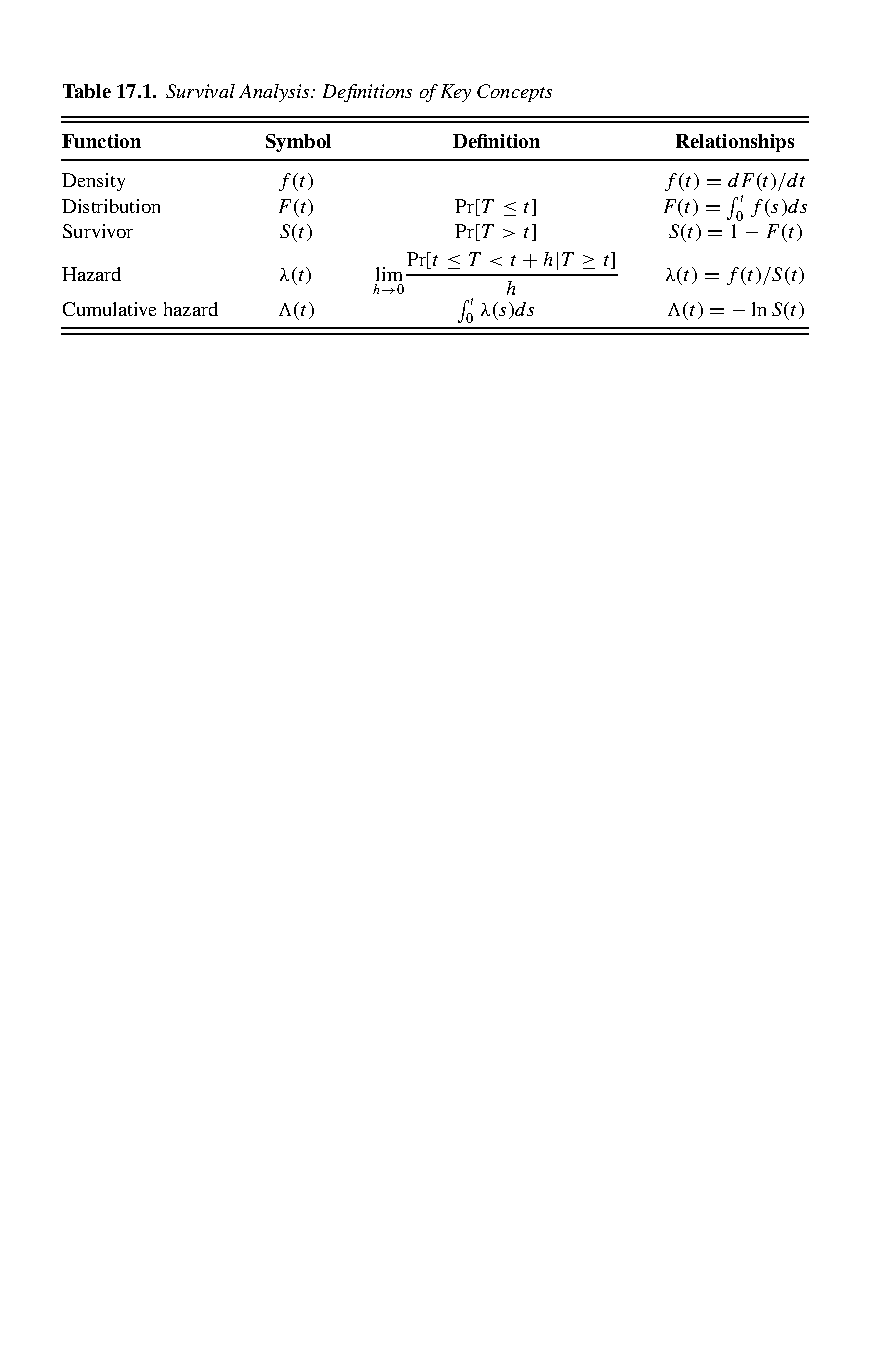
\includegraphics[width=4.5in]{./resources/parametrictable1.pdf}
\end{center}
\end{frame}

\begin{frame}
\frametitle{What about Discrete Time?}
\begin{itemize}
\item Maybe we only see survival annually/weekly/etc. not actual failure time.
\item Basic idea is the same. Have to be careful about ties. Divide failures into $t_j$ buckets
\begin{eqnarray*}
\lambda_j &=& Pr[T = t_j | T \geq t_j] = f^d(t_j) / S^d(t_{j-})\\
\Lambda^d(t)&=&\sum_{j | t_j \leq t} \lambda_j \\
S^d &=& Pr [T \geq t ] = \prod_{j| t_j \leq t} (1-\lambda_j)
\end{eqnarray*}
\item Can define the \alert{product integral} which is regular product in discrete case and exponential of integral in continuous case.
\end{itemize}
\end{frame}



\begin{frame}
\frametitle{Nonparametric estimation}
\begin{itemize}

\item Without censoring, things are easy: just let
\[
\hat{S}(t)=\frac{1}{n}\sum_{i=1}^n \mathbf{1} (T_i \geq  t).
\]
\item if you want a smooth hazard function, take a smooth estimator, e.g.
(with some ``small'' bandwidth $w>0$)
\[
\hat{S}(t)=\frac{1}{n}\sum_{i=1}^n \frac{1}{1+\exp((t-T_i)/w)},
\]
\item and then take minus the derivative of the log of this estimate.
\end{itemize}
\alert {What if there is censoring?} Kaplan-Meier!
\end{frame}


\begin{frame}
\frametitle{Kaplan-Meier}
\begin{itemize}
\item We define the
ordered durations as 
\[
T_{(1)} < \ldots < T_{(n)},
\]
\item let $d_j$ be the number of observations $i$ for which $T_i=T_{(j)}$
\item Let $m_j$ number of spells censored in $[t_j,t_{j+1})$
\item and $r_j$ the cardinality of the \alert{risk set}  at duration $t_{j-}$   $r_j=\sum_{l | l \geq j} d_l + m_l$
\item Simple estimate of the hazard function $\hat{\lambda}_j = \frac{d_j}{r_j}$.
\item Kaplan-Meier estimator  of the survival function is the \alert{Product Limit Estimator}
\[
\hat{S}(t)=\Pi_{j|t_j \leq t} \left(
1-\frac{d_j}{r_j}
\right) = \Pi_{j|t_j \leq t} \left(
\frac{r_j- d_j}{r_j}
\right)
\]
\item It is normally distributed (asymptotically), with (Greenwood) variance
\[
\hat{V}[\hat{S}(t)]=(\hat{S}(t))^2 \cdot \sum_{j|t_j \leq t}
\frac{d_j}{r_j(r_j-d_j)}.
\]
\end{itemize}
\end{frame}

\begin{frame}
\frametitle{Other stuff}
Think about what happens when $m_j= 0$ (no censoring)
\begin{itemize}
\item $r_j=\sum_{l | l \geq j} d_l + m_l \rightarrow r_{j+1} = r_j - d_j$.
\item $ \hat{S}(t)= \Pi_{j|t_j \leq t} \left( \frac{r_j- d_j}{r_j} \right) =  \Pi_{j|t_j \leq t} \frac{r_{j+1}}{r_j} = \frac{r_j}{N}$
\item Again -- exactly what we would expect -- one minus the ECDF.
\end{itemize}
How do we deal with ties?
\begin{itemize}
\item Lots of ties can create problems. Implicitly we assume all deaths are at same time in period.
\item Why does this matter-- well how many are remaining in $r_j$?
\item $r_j$ is potentially biased if we have lots of ties.
\item Can either try corrections or sample data at higher frequency
\end{itemize}
\end{frame}



\begin{frame}
\frametitle{Exponential and Weibull }
\begin{itemize}
\item The exponential is popular because it has a \alert{constant hazard rate} $\lambda(t) =\gamma$ which does not depend on $t$.
\item This is often referred to as the \alert{memorylessness} property of the exponential.
\item This is analytically convenient but it makes it hard to fit things in practice (you only have one parameter!)
\item The Weibull is a generalization with $\lambda(t) = \gamma \alpha t^{\alpha-1}$. For $\alpha=1$ we have exponential.
\item For $\alpha > 1$ i is increasing and for $\alpha < 1$ it is decreasing (monotonically). 
\item Weibull used to be popular in econometrics for simple parametric analysis.
\end{itemize}
\end{frame}



\begin{frame}
\frametitle{Exponential and Weibull }
\begin{center}
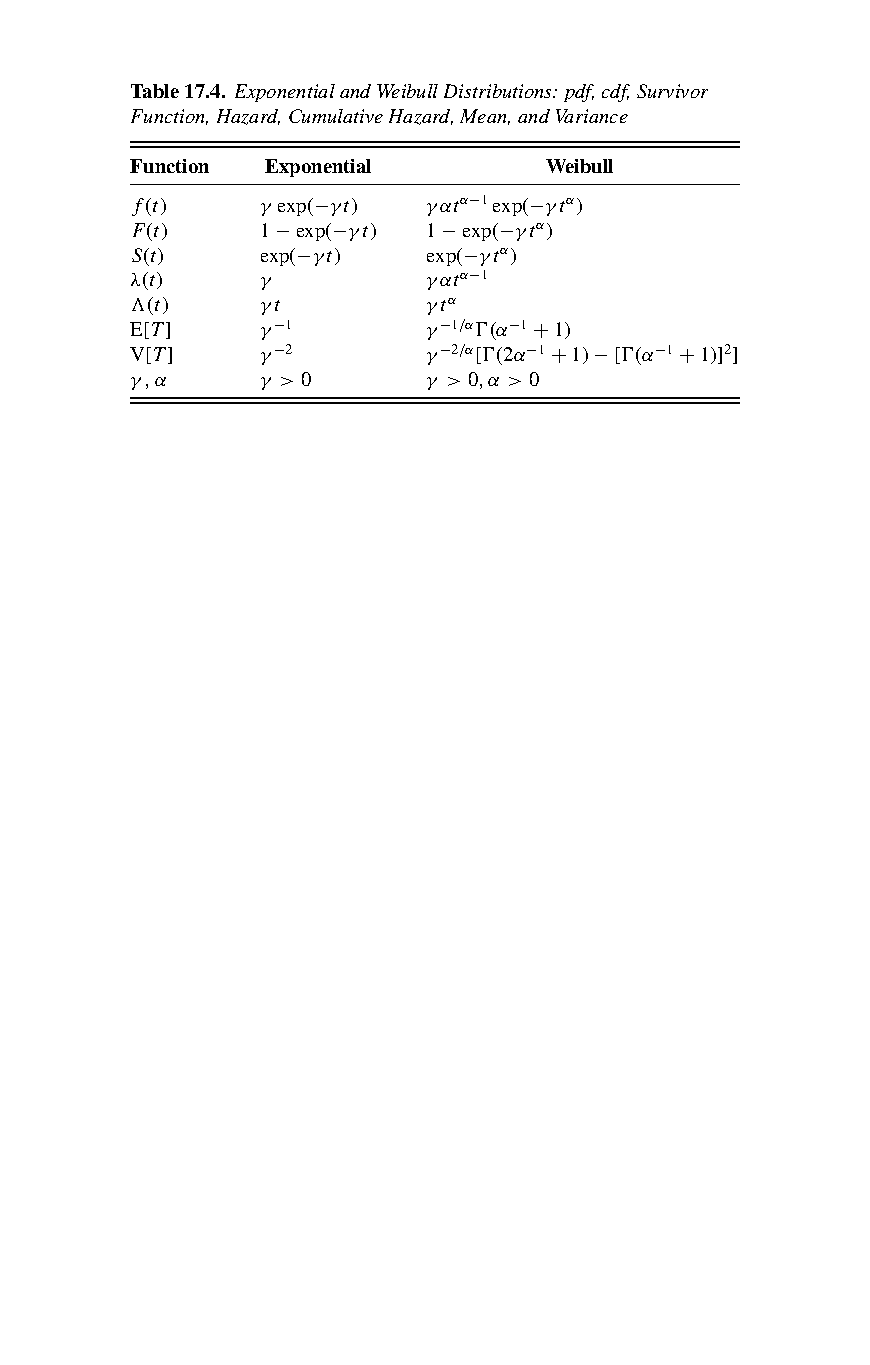
\includegraphics[width=4.5in]{./resources/figure17-4.pdf}
\end{center}
\end{frame}


\begin{frame}
\frametitle{Comparison of Parametric Models}
\begin{center}
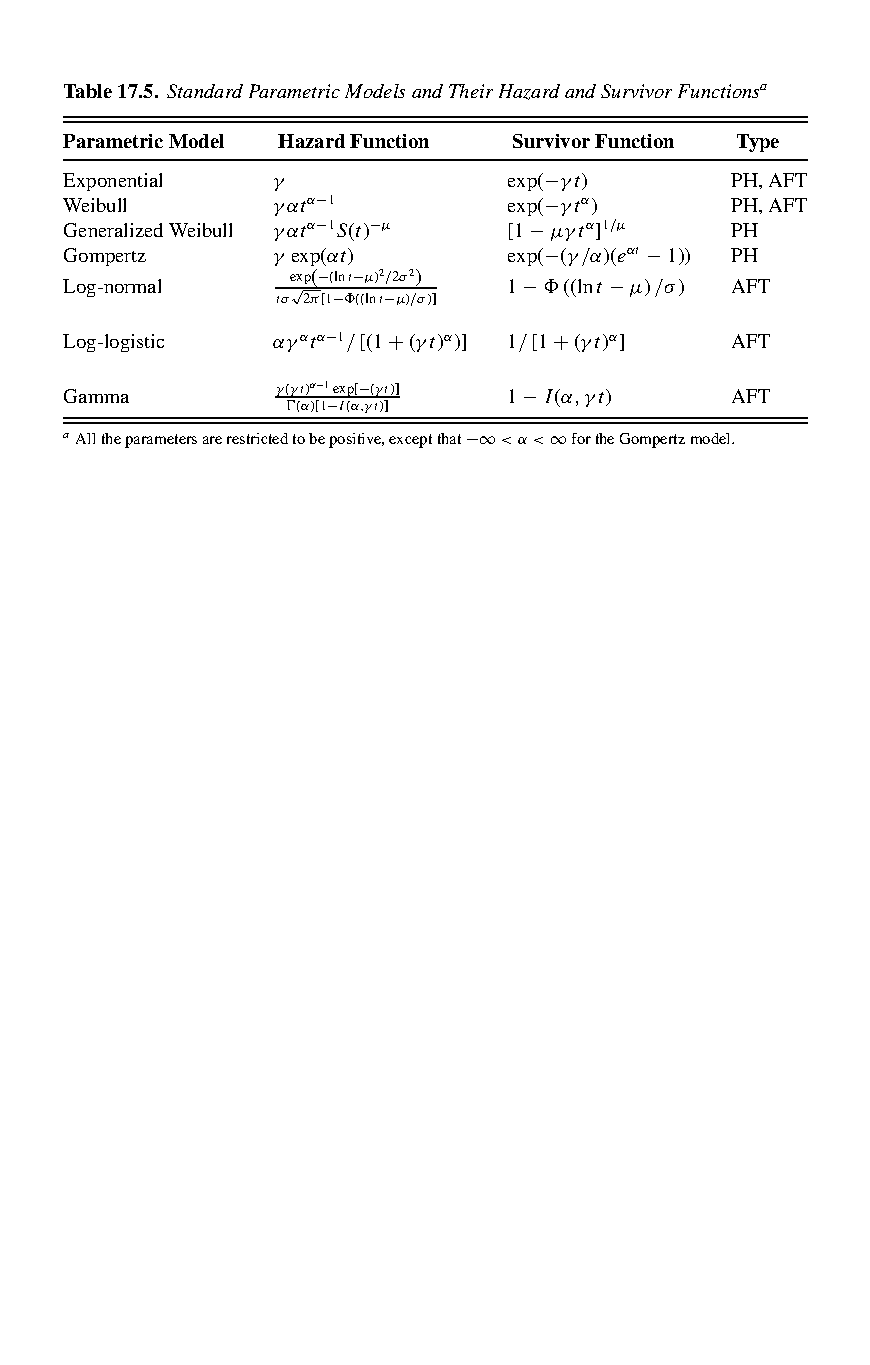
\includegraphics[width=4.5in]{./resources/figure17-5.pdf}
\end{center}
\end{frame}

\begin{frame}
\frametitle{Adding Covariates }
\begin{itemize}
\item We can also add covariates by letting $\gamma = \beta X$.
\item Sometimes this is called \alert{link function} or \alert{generalized linear models} similar to what we saw with the logit or probit.
\item It is usually a bad idea to link more than one nonlinear parameter this way.
\item We would typically estimate via MLE. Writing down the full-data log-likelihood is straightforward.
\item A frequently used special-case are \alert{proportional hazard models}
\end{itemize}
\end{frame}




\begin{frame}
\frametitle{The Proportional Hazard  Model}
With covariates $x$, the hazard function is $h(t \vert x)$; we specify
\[
\lambda(t \vert x)=\lambda_0(t)\phi(x).
\]
\begin{itemize}
\item $\lambda_0$ and $\phi$ are up to a positive multiplicative constant.)
\item  We call $\lambda_0$ the \alert{ baseline hazard}; every individual has
a hazard that is just a proportional version of the baseline hazard.
\end{itemize}
The baseline hazard could be:
\begin{itemize}
\item constant: the survival function is exponential
\item a power function $\lambda_0(t)=\gamma t^{\alpha}$; e.g. for
$\alpha<0 $ we have \alert{negative duration dependence} (the
long-term unemployed\ldots)
\item more complicated (flexible) specifications.
\end{itemize}
\end{frame}



\begin{frame}
\frametitle{Estimating the PH Model}
{\bf Maximum likelihood:} works for any parametric modelx
$\lambda(t \vert x,\beta)$ of the full hazard function;\\
(here: w/o censoring, without corrleation across individuals):
\[
\max_{\beta} \sum_{i=1}^n \ln f(T_i \vert x_i,\beta),
\]
where $f(t \vert x,\beta)$ is the density of the duration $T$ induced by
$\lambda$:
\[
f(t \vert x)=\lambda(t \vert x)S(t \vert x)=\lambda(t \vert x)\exp(-\Lambda(t \vert x)),
\]
so the log-likelihood for $i$ is just $\ln
\lambda(T_i \vert x_i,\beta)-\Lambda(T_i \vert x_i,\beta)$.
\end{frame}

\begin{frame}
\frametitle{What's the point?}
\begin{itemize}
\item The (partial) additive separability of the log-likelihood in the PH model is designed to make our lives easier.
\item Presumably, we specified $\lambda$ so that its integral $\Lambda$ is easy to
compute. 
\item For PH: the log-likelihood for $i$ is:\\
$\ln \lambda_0(T_i,\beta)+\ln\phi(x_i,\beta)-\Lambda_0(T_i,\beta)\phi(x_i,\beta)$.
\item The most common choice is $\phi(x_i,\beta) = \exp(x_i \beta)$ so that $\ln\phi(x_i,\beta) = x_i \beta$.
\item In that case we have that $\partial \lambda/ \partial x_j = \beta_j \cdot \lambda$.
\item One remaing problem: what to do with the baseline hazard function (is that even identified?).
\end{itemize}
\end{frame}

\begin{frame}
\frametitle{Cox's Partial Likelihood for the PH Model}
\begin{itemize}
\item if we do not want to assume anything about the shape of the \alert{baseline hazard function}
\item but we are happy specifying $\phi(x,\beta)$
\item then we will only look at the {\em order\/} of the durations: we
reorder individuals so that $T_{i_1}<\ldots<T_{i_n}$
\item \ldots and we forget about the durations! Then the partial
likelihood is:
\[
\sum_{j=1}^n
\left(
 \ln \phi(x_{i_j},\beta)
  -\ln
  \left(
  \sum_{l=j}^n
\phi(x_{i_l},\beta)
\right)
\right).
\]
\item This is a \alert{limited information maximum likelihood estimator}. It is not fully efficient!
\item But it may be robust to mis-specifying $\lambda_0$.  Is it actually a valid likelihood? \alert{not sure!}.
\end{itemize}
\end{frame}

\begin{frame}
\frametitle{How did that work?}
Once we have ordered everything:
\begin{itemize}
\item Let $R(t_j)$ be the set of spells at risk (still alive) at $t_j$
\item $d_j$ are the deaths at time $t_j$ $\sum_l \mathbf{1}[t_l = t_j]$.
\item Consider only at-risk spells ending a fixed $t_j$
\begin{eqnarray*}
Pr[T_j = t_j \vert R(t_j)] &=& \frac{Pr[T_j = t_j \vert T_j \geq t_j]}{\sum_{l \in R(t_j)} Pr[T_l = t_l \vert T_l \geq t_j]}\\
 &=& \frac{\lambda_j(t_j | x_j, \beta) ]}{\sum_{l \in R(t_j)} \lambda_l (t_j,x_l,\beta)}\\
 &=& \frac{\phi( x_j, \beta) }{\sum_{l \in R(t_j)} \phi (x_l,\beta)}\\
\end{eqnarray*}
\item $\lambda_0$ drops out because of PH.
\end{itemize}
\end{frame}

\begin{frame} 
\frametitle{Why?}
\begin{itemize}
\item \emph{Intuition:\/} those individuals who exit first are (on average) those in
the risk set whose covariates $x$ give them the largest $\phi(x,\beta)$.
\item After we have $\hat{\beta}$ we can estimate the baseline integrated
hazard; denoting $N(t)$=number of individuals with $T=t$
\[
\widehat{\Lambda_0}(T_{i_j})=\sum_{m=1}^j \frac{N(T_{i_m})}{\sum_{l=m}^n
\phi(x_{i_l},\hat{\beta})}.
\]
\end{itemize}
\end{frame}


\begin{frame}
\frametitle{Tricks}

{\em A simple way to test the model}:
\begin{itemize}
\item just take two different groups of individuals, estimate PH on each, check whether the baseline
hazards look \alert{proportional} \textbf{NOT} \alert{equal}
\end{itemize}

 {\em testing a  parametric specification of the baseline
hazard $\bar{\Lambda}_0$:} 
\begin{itemize}
\item define  generalized residuals $\bar{u}_i=\bar{\Lambda_0}(T_i)$
\item Under the true  model, for any $z$
\[
\Pr(\bar{u} <z) \simeq
\Pr(T_i<\bar{\Lambda}_0^{-1}(z))=1-S_0(\bar{\Lambda}_0^{-1}(z)).
 \]
\item it should be $1-\exp(-z)$ if $S_0=\exp(-\bar{\Lambda}_0)$.
\item So you can estimate the integrated hazard of
 $(\bar{u}_1,\ldots,\bar{u}_n)$; it should be $\Lambda_u(z) \equiv z$.
\end{itemize}
\end{frame}


\begin{frame}
\frametitle{The PH Model is Usually too Restrictive}
\begin{itemize}
\item {\bf Fact:}  the hazard rate of leaving unemployment decreases
in time;
\item It could be {\em skimming}: the more able, more willing, better
connected find a job faster;
\item or it could be ``technological'': skills deteriorate over time.
\item Under the PH model it can only be the latter: negative duration
dependence. $\rightarrow$ introduce unobserved heterogeneity:
\[
\lambda(t \vert x,v)=\lambda_0(t)\phi(x) v.
\]
\item $v$ is a ``type'' that is unobserved by the econometrician; we
only assume that it is uncorrelated with $x$ and independent of $t$.
\end{itemize}
\end{frame}

 \begin{frame}
 \frametitle{Dynamic selection}
\begin{itemize}
\item The model with $v$ is called the \textbf{Mixed PH model} (MPH).
\item In the unemployment story: the larger $v$'s have a higher hazard
  rate, so they find a job faster
\item Over time, the distribution of $v$ moves (stochastically) to the
  left.
\item This \alert{dynamic selection} is a general phenomenon in the MPH
  model: $\lambda(t \vert x)$ has ``more negative duration dependence'' than
  $\lambda(t \vert x,v)$.
\item Can we test dynamic selection vs true negative duration dependence
  ($\lambda_0$ decreasing)? $\rightarrow$ identification issues.
  \item This idea shows up in dynamic models of durable goods purchases as well.
  \end{itemize}
\end{frame}



\begin{frame}
\frametitle{Identification}
We still can recover the aggregate survival function from the data, but now it
is a mixture:
\[
S^A(t \vert x)=\Pr(T \geq t \vert x)=
\int \exp(-v \phi(x)\Lambda_0(t))dF(v).
\]
\begin{itemize}
\item Can we recover $\phi$ and $\lambda_0$ without assuming anything on $F$?
\item Almost \ldots\ in theory: we just need to assume that $E(v)$ is finite.
\end{itemize}
\end{frame}



\begin{frame}
\frametitle{A Constructive Proof, 1}
\begin{itemize}
\item Normalize $Ev=1$; and $\phi(x_0)=1$ for some $x_0$. 
\item Then the aggregate hazard function is
\[
\lambda^A(t \vert x)=-\frac{\partial \log S^A}{\partial t}(t \vert x)
\]
that is
\[
\frac{\int v \phi(x)\lambda_0(t)\exp(-v \phi(x)\Lambda_0(t))dF(v)}{S^A(t \vert x)}.
\]
\item
Look at $x=x_0$ and $t=0^+$: then $\Lambda_0(t) \simeq 0$, so
\[
\lambda^A(0^+\vert x_0)=\frac{Ev \times k(x_0) \times \lambda_0(0)}{S^A(0\vert x_0)}=\lambda_0(0).
\]
\item
and
\[
\phi(x)=\frac{\lambda^A(0^+ \vert x)}{\lambda^A(0^+ \vert x_0)}.
\]
\end{itemize}
\end{frame}

\begin{frame}
\frametitle{A Constructive Proof, 2}
\begin{itemize}
\item Now we can define
\[
m^A(t \vert x)=-\frac{\partial \log S^A(t,x)}{\partial \phi(x)}
\]
\item and we get the baseline hazard from 
\[
\frac{\lambda_0(t)}{\Lambda_0(t)}=\frac{\lambda^A(t \vert x)}{m^A(t \vert x)};
\]
\item  and we can also recover $F$. 
\item In practice we would specify functional forms of course.
\end{itemize}
\end{frame}


\begin{frame}
\frametitle{Is that Practical?}
\begin{itemize}
\item We are relying heavily on ``identification at 0'': that is where we
get $\phi(x)$, the rest depends on it.
\item Empirical researchers have found that it is often a slim basis (and a
very slow-converging estimator)---but
anything else will be parametric.
\item The alternative is to use richer data: multiple durations/multiple spells. 
\end{itemize}
\end{frame}

\begin{frame}
\frametitle{Application 1: job search}
E.g. Cahuc/Postel-Vinay-Robin, {\em Econometrica \/} 2006.
\begin{itemize}
\item Workers are heterogeneous, so are firms; 
\item a worker quits when he gets a better outside offer (exogenous Poisson($\lambda$)).
\item We observe (given matched employer-employee data): 
\begin{itemize}
\item job durations (how long each worker stays in a job)
\item and distributions of wages (mostly) across firms.
\end{itemize}
\end{itemize}
\end{frame}


\begin{frame}
\frametitle{Bad luck}
\begin{itemize}
\item The likelihood for the duration of job spells is independent of heterogeneity!
\[
f(t)=\frac{\delta(\delta+\lambda)}{\lambda}\int_{\delta t}^{(\delta+\lambda)t} \frac{\exp(-x)}{x} dx.
\]
\item So we can identify $\lambda$ and $\delta$, and nothing about heterogeneity of firms and workers.
\item (But the good thing is that we don't need to assume anything about it and we get $\delta$ and $\lambda$).
\end{itemize}
\end{frame}

\begin{frame}
\frametitle{Better luck}
\begin{itemize}
\item Given bargaining on wages, outside options matter;
\item and outside options generate option values, which increase with heterogeneity ( volatility!).
\item ``So'' by looking at the distribution of wages we can infer heterogeneity.
\end{itemize}
\end{frame}



\begin{frame}
\frametitle{Application 2: moral hazard in insurance}
Abbring-Chiappori-Pinquet, {\em JEEA\/} 2003.
\begin{itemize}
\item Insurees have exogenous  types (risk) $v$ that are unobserved; we call this adverse selection;
\item they also decide to adopt a risky behavior or not: \alert{moral hazard}.
\item Data typically gives us a series of claims for each individual. 
\item A state could be: ``I have had exactly $p$ claims so far'' and a spell is the time between two claims.
\end{itemize}
\end{frame}


\begin{frame}
\frametitle{Duration dependence}
\begin{itemize}
\item Adverse selection induces positive duration dependence: the time between claims is positively correlated.
\item On the other hand, with experience rating a claim (at fault) increases premia and makes risky behavior more costly---typically
\item so moral hazard induces negative duration dependence.
\item How can we test for the latter while controlling for the former?
\end{itemize}
\end{frame}


\begin{frame}
\frametitle{The Model}
\begin{itemize}
\item The hazard function for claim $(p+1)$ at $t$, given state $p$, is (dropping $x$)
\[
v h_0(t) A^{-p},
\]
\item  with $A$ and $h_0$ unknown. 
\item $v$ models exogeneous unobserved risk, 
\item every time a claim occurs, the hazard for the next claim is divided by  $A$: moral hazard.
\item It is the MPH, with a twist: the $p$.
\end{itemize}
\end{frame}


\begin{frame}
\frametitle{Estimating Finite Mixtures}
\begin{itemize}
\item In practice estimating finite mixture models can be tricky.
\item A simple example is the mixture of normals (incomplete data likelihood)
\begin{eqnarray*}
f(x_1,\ldots,x_n | \theta) = \prod_{i=1}^N \sum_{k=1}^K \pi_k f(x_i | \mu_k, \sigma_k)
\end{eqnarray*}
\item We need to find both mixture weights $\pi_k = Pr(z_k)$ and the components $(\mu_k,\sigma_k)$ the weights define a valid probabiltiy measure $\sum_k \pi_k = 1$.
\item Easy problem is \alert{label switching}. Usually it helps to order the components by say decreasing $\pi_1 > \pi_2 > \ldots$ or  $\mu_1 > \mu_2 > \ldots$ 
\item The real problem is that which component you belong to is unobserved. We can add an extra indicator variable $z_{ik} \in \{0,1\}$.
\item We don't care about $z_{ik}$ per-se so they are \alert{nuisance parameters}.
\end{itemize}
\end{frame}

\begin{frame}
\frametitle{Estimating Finite Mixtures}
\begin{itemize}
\item We can write the complete data log-likelihood (as if we observed $z_{ik}$):
\begin{eqnarray*}
l(x_1,\ldots,x_n | \theta) = \sum_{i=1}^N  \log \left( \sum_{k=1}^K I[z_i = k]  \pi_k f(x_i \mu_k, \sigma_k) \right)
\end{eqnarray*}
\item We can instead maximized the expected log-likelihood where we take the expectation $E_{z|\theta}$
\begin{eqnarray*}
\alpha_{ik}(\theta) = Pr(z_{ik} =1 | x_i,\theta) = \frac{f_k(x_i,z_k,\mu_k,\sigma_k) \pi_k }{\sum_{m=1}^K f_m(x_i,z_m,\mu_m,\sigma_m) \pi_m}
\end{eqnarray*}
\item Now we have a probability $\hat{\alpha}_{ik}$ that gives us the probability that $i$ came from component $k$. We also compute $\hat{\pi}_k = \frac{1}{N} \sum_{i=1}^N \alpha_{ik}$
\end{itemize}
\end{frame}

\begin{frame}
\frametitle{EM Algorithm}
\begin{itemize}
\item Treat the $\hat{\alpha}_k(\theta^{(q)})$ as data and maximize to find $\mu_k,\sigma_k$ for each $k$
\begin{eqnarray*}
\hat{\theta}^{(q+1)} = \arg \max_{\theta}  \sum_{i=1}^N  \log \left( \sum_{k=1}^K \hat{\alpha}_k(\theta^{(q)}) f(x_i | z_{ik}, \theta ) \right)
\end{eqnarray*}
\item We iterate between updating $\hat{\alpha}_k(\theta^{(q)})$ (E-step) and $\hat{\theta}^{(q+1)}$ (M-step)
\item For the mixture of normals we can compute the M-step very easily:
\begin{eqnarray*}https://en.wikipedia.org/wiki/Jensen%27s_inequality#General_inequality_in_a_probabilistic_setting
\mu_k^{(q+1)} &=& \frac{1}{N} \sum_{i=1}^N \hat{\alpha}_k(\theta^{(q)}) x_{i}\\
\sigma_k^{(q+1)} &=& \frac{1}{N} \sum_{i=1}^N \hat{\alpha}_k(\theta^{(q)}) (x_{i} - \overline{x})^2 \\
\end{eqnarray*}
\end{itemize}
\end{frame}

\begin{frame}
\frametitle{EM Algorithm}
\begin{itemize}
\item EM algorithm has the advantage that it avoids complicated integrals in computing the expected log-likelihood over the missing data.
\item For a large set of families it is proven to converge to the MLE
\item That convergence is \alert{monotonic} and \alert{linear}. (Newton's method is quadratic)
\item This means it can be slow, but sometimes $\nabla_{\theta} f (\cdot)$ is really complicated.
\end{itemize}
\end{frame}

\section*{Thanks!}

\end{document}